\section{Annotation, Files and Protocol}
\subsection{Data Statistics}
MSU-PID includes two subsets, one for each plant type: Arabidopsis and bean.
The statistic information of these two subsets are summarized in Table~\ref{tab:stat}.
The images were acquired every hour.
As there is no light at night hours, plants can not be imaged by the fluorescence and RGB color sensors while IR and depth cameras can still perform the capturing during the night.
In order to make sure that all four modalities are present at the same time, we release the part of images captured only in the day hours, which are $15$ images per day for Arabidopsis and $13$ for bean for all four modalities.

The two subsets differ in image resolutions.
As shown in Figure~\ref{fig:fourmodality}, we grow and image a single bean plant while a whole tray of Arabidopsis are grown at the same time.
Therefore, the resolution of a Arabidopsis image is much lower than that of a bean image.
We manually crop $16$ Arabidopsis plants, which have been captured by all three cameras simultaneously.
Table~\ref{tab:resolution} summaries the image resolution of each plant in all four modalities.


\begin{figure*}
\centering
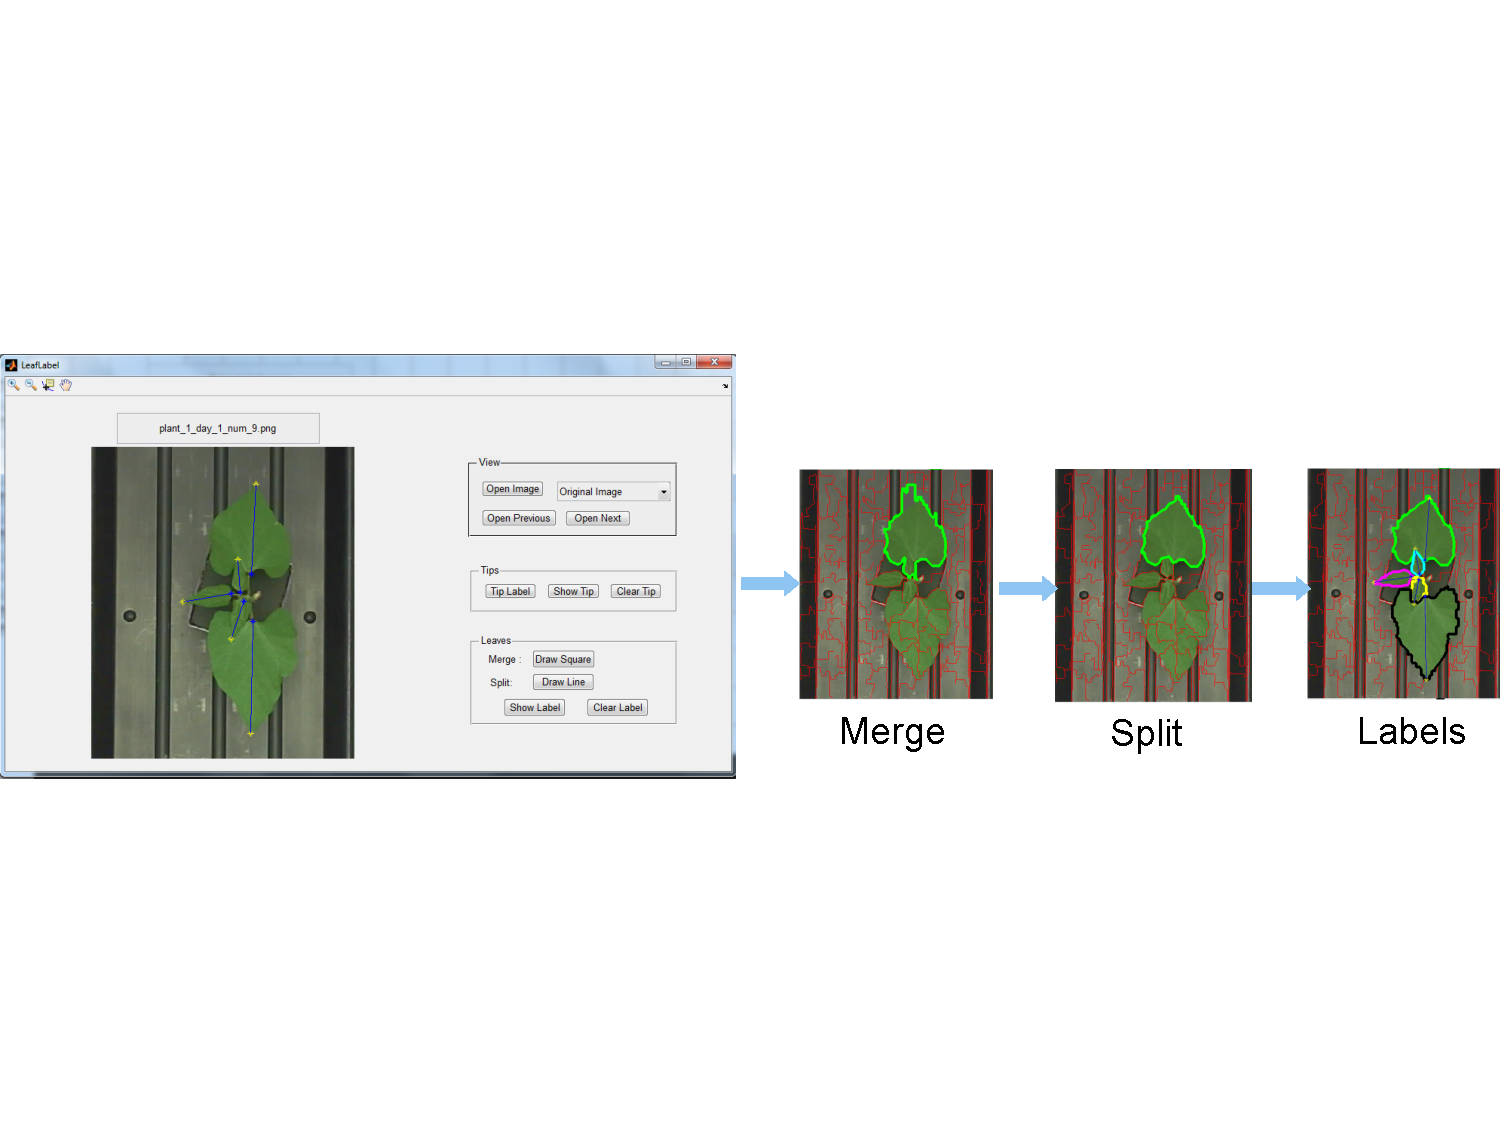
\includegraphics[width=.90\textwidth]{Figures/labeling}\\
\caption{Leaf labeling process, including tip labels and leaf segmentation annotation.}
\label{fig:label}
\end{figure*}

%\begin{figure*}
%\begin{centering}
%\begin{tabular}{@{}c@{} c@{} c@{} c@{} c@{} c@{} c@{} c@{} c@{}}
%%\begin{tabular}{lllllllll}
%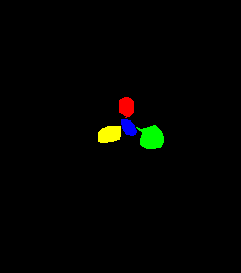
\includegraphics[width=.11\textwidth]{Figures/labelExample/plant_1_day_1_num_13.png}&
%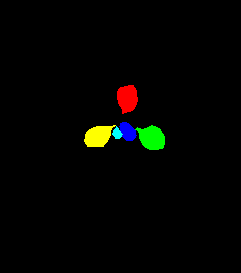
\includegraphics[width=.11\textwidth]{Figures/labelExample/plant_1_day_2_num_13.png}&
%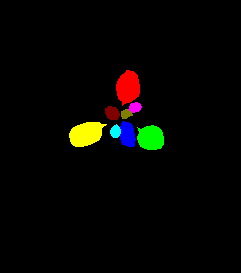
\includegraphics[width=.11\textwidth]{Figures/labelExample/plant_1_day_3_num_13.png}&
%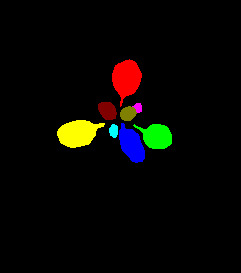
\includegraphics[width=.11\textwidth]{Figures/labelExample/plant_1_day_4_num_13.png}&
%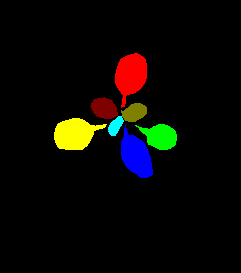
\includegraphics[width=.11\textwidth]{Figures/labelExample/plant_1_day_5_num_13.png}&
%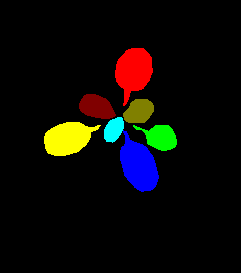
\includegraphics[width=.11\textwidth]{Figures/labelExample/plant_1_day_6_num_13.png}&
%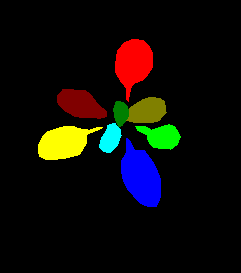
\includegraphics[width=.11\textwidth]{Figures/labelExample/plant_1_day_7_num_13.png}&
%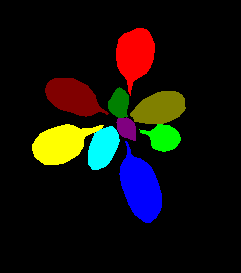
\includegraphics[width=.11\textwidth]{Figures/labelExample/plant_1_day_8_num_13.png}&
%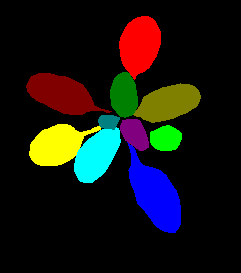
\includegraphics[width=.11\textwidth]{Figures/labelExample/plant_1_day_9_num_13.png}\\
%day 1 & day 2 & day 3 & day 4 & day 5 & day 6 & day 7 & day 8 & day 9 \\
%\end{tabular}
%\caption{Leaf labeling results of one Arabidopsis plant over nine days with one image per day. Note that the labels of tips are not shown for visualization clarity. }
%\label{fig:LabelExample}
%\end{centering}
%\end{figure*}

It is often argued which is the best setting due to the trade-off between the image resolution and the throughput of phenotyping experiments.
We chose to image a whole tray of Arabidopsis at lower resolution rather than an individual at higher resolution, because it better reflects high-throughput protocols, which in practice allows direct comparison of multiple genotypes in the same experiment.
In contrary, we chose to image a single bean plant because we anticipate enabling development of $3$D plant canopy reconstruction algorithms for bush plants.


\subsection{Manual Annotations}
\label{sec:annotation}
Part of the database is manually annotated to provide ground truth tip locations, leaf segmentation results, and leaf consistency overtime.
We use the fluorescence images as the input for labeling because of their clean and uniform background.
%Tip locations are saved in a TXT file for each frame.
%Leaf segmentation results are stored in a PNG image for each frame with one color for each leaf.
%The same color is used to represent the same leaf over a sequence of frames.

For Arabidopsis images, we label $4$ frames each day.
While for bean images, we label $7$ frames each day because of their spontaneous and fast leaf movement.
A Matlab GUI interface is developed for leaf labeling, as shown in Figure~\ref{fig:label}, which will also be available to the public.
A user can open a plant image (``Open") to label the two tips and annotate each leaf segment.
The results will be automatically saved once a user moves to a previous or next image (``Previous", and ``Next").
For consistent annotation of the same leaf over time, we show a number on the center of each leaf indicating the order of labeling from the previous frame.

The labeling of the leaf segment (``Leaf Label") is implemented by clicking the boundary of one leaf at each time.
In order to provide more accuracy labeling, we click very dense points ($\sim20$ points on average for each leaf) on the boundary.
The labeled leaf boundary is overlaid on the image for better visualization to guide the next action.
Incorrect label can be deleted right after the labeling by clicking ``Clear".
All leaf labels can be deleted by clicking ``Clear All".
This process continues until all leaf segments have been annotated.
Once a leaf is invisible due to occlusion, the label can be skipped by clicking ``Invisible".

The labeling of leaf tips (``Tip Label") is implemented by clicking pairs of points on the image.
The outer tip is always clicked first before the inner tip.
For visualization, a line connecting each pair of tips will be shown immediately after clicking the inner tip.
Inaccurate labels can be deleted by clicking the right button of the mouse near the labeled point and relabeled by clicking the left button again immediately after deletion.
All tips can be deleted by clicking ``Clear Tip" and relabel again.
The ``Show Tip" option is to select whether to show the tips or not.
For relabeling of both leaf segments and leaf tips on the current image, click ``Restart".

After the labeling, we visually go through the results and correct inaccurate labels.
One example of the labeling results for one plant is shown in Figure~\ref{fig:trackExample} $(b)$, where one color is used to represent each specific leaf.
As we can see during the transition between day $5$ and day $6$, there is one leaf showing up and covering up the leaf underneath, which disappears and will not be annotated later.
% In total, we labeled $5,142$ leaves for fluorescence images.

Note that one alternative approach for labeling leaf segments is to directly label the membership of superpixels instead of drawing a polygon along the boundary.
Our experience is that since a noticeable percentage of extracted superpixels cover pixels of two neighboring leaves, the extra effort of breaking a super pixel into two makes it a less efficient alternative.


\subsection{Multimodal Annotations}
\begin{figure*}[t]
\begin{centering}
\begin{tabular}{cccc}
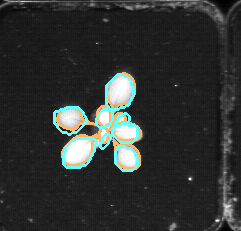
\includegraphics[width=.15\textwidth]{Figures/LabelAlignment/day_3_hour_23-seg_ir.png}&
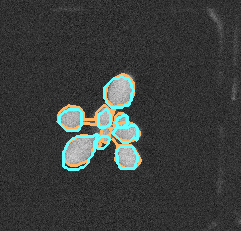
\includegraphics[width=.15\textwidth]{Figures/LabelAlignment/day_3_hour_23-seg_fmp.png}&
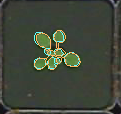
\includegraphics[width=.15\textwidth]{Figures/LabelAlignment/day_3_hour_23-seg_rgb.png}&
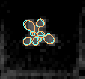
\includegraphics[width=.15\textwidth]{Figures/LabelAlignment/day_3_hour_23-seg_depth.png}\\
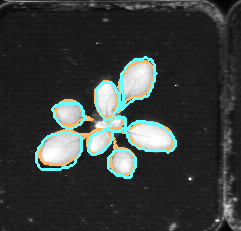
\includegraphics[width=.15\textwidth]{Figures/LabelAlignment/day_5_hour_23-seg_ir.png}&
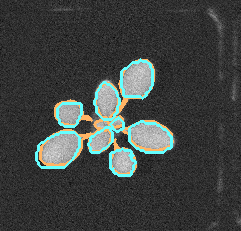
\includegraphics[width=.15\textwidth]{Figures/LabelAlignment/day_5_hour_23-seg_fmp.png}&
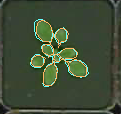
\includegraphics[width=.15\textwidth]{Figures/LabelAlignment/day_5_hour_23-seg_rgb.png}&
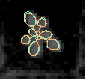
\includegraphics[width=.15\textwidth]{Figures/LabelAlignment/day_5_hour_23-seg_depth.png}\\
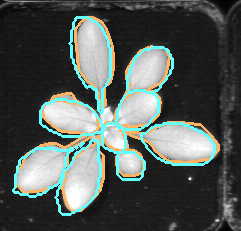
\includegraphics[width=.15\textwidth]{Figures/LabelAlignment/day_9_hour_20-seg_ir.png}&
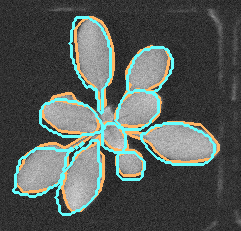
\includegraphics[width=.15\textwidth]{Figures/LabelAlignment/day_9_hour_20-seg_fmp.png}&
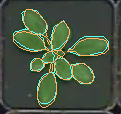
\includegraphics[width=.15\textwidth]{Figures/LabelAlignment/day_9_hour_20-seg_rgb.png}&
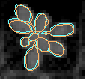
\includegraphics[width=.15\textwidth]{Figures/LabelAlignment/day_9_hour_20-seg_depth.png}\\
($a$) & ($b$) & ($c$) & ($d$) \\
\end{tabular}
\caption{Label propagation between all four modalities ($a$) IR, ($b$) fluorescence, ($c$) RGB color, and ($d$) depth, of a sample plant in the Arabidopsis collection for day $3$ (top row), day $5$ (middle row), and day $9$ (bottom row).
In the dataset the manual segmentation is performed on the fluorescence images and is outlined here as orange lines propagated to all modalities (i.e., the orange lines in (b) are manual labels while these in other three modalities are propagated labels).
The IR images are taken by the same camera and so will have exact pixel correspondence.
To assess the segmented pixel propagation to other modalities, we also manually labeled a subset of the color plant images (shown as cyan in (c)) and propagated this label to other three modalities (i.e., the cyan in (a,b,d) are propagated labels).
Comparing these boundaries in each modality gives a measure of the propagation errors due to parallax, and we provide quantitative analysis in Table~\ref{tab:labelError}.
Note that the color and depth images are rotated $90$ degrees.}
\label{fig:LabelAlignment}
\end{centering}
\end{figure*}


\begin{table*}[t]
\centering
\caption{Human label performance vs. label propagation performance.
$L_1$ and $L_2$ are the manual label results from two annotators, and $L_t$ is the propagated results.
The {\it{SBD}} score is averaged over $3$ plants.}
\begin{tabular}{c|c|c|c|c|c|c}
\hline
    & \multicolumn{3}{c|}{fluorescence modality} & \multicolumn{3}{c}{RGB modality}\\ \hline
    & $L_1$ vs. $L_1$ & $L_1$ vs. $L_2$  & $L_1$ vs. $L_t$ & $L_1$ vs. $L_1$ & $L_1$ vs. $L_2$ & $L_1$ vs. $L_t$ \\ \hline
   day$\_3\_$hour$\_23$ & $1$ & $0.808$ & $0.804$ & $1$ & $0.827$ & $0.802$ \\ \hline
   day$\_5\_$hour$\_23$ & $1$ & $0.830$ & $0.836$ & $1$ & $0.871$ & $0.837$ \\ \hline
   day$\_9\_$hour$\_20$ & $1$ & $0.903$ & $0.886$ & $1$ & $0.877$ & $0.789$ \\ \hline
                   average &          $1$ & $0.847$ & $0.842$ & $1$ & $0.858$ & $0.809$ \\ \hline
\end{tabular}
\label{tab:labelError}
\end{table*}

The leaf labeling can be propagated from the fluorescence images to each of the other modalities for the Arabidopsis sequences.
To do this, we approximate a plant image with a plane, and estimate homographies that transform the fluorescence images into the images in other modalities.
This provides a direct mapping of the pixel labels between each modality.
% and is illustrated in Figure~\ref{fig:LabelAlignment}.

To quantify the precision of the label propagation, we manually label $3$ images for each of $3$ Arabidopsis plants ($9$ images in total) on fluorescence and RGB modalities.
The labels in each modality is propagated on other modalities.
The result of one plant is illustrated in Figure~\ref{fig:LabelAlignment}.
This mapping will introduce errors due to depth-based parallax.
We use {\it{SBD}} score, which will be introduced in Section~\ref{sec:protocol}, to evaluate the similarity between the manual labels and the propagated labels.
In order to compute the inter-annotators variability, we ask two different annotators to label the same $9$ images and compute the {\it{SBD}} score.
The results are shown in Table~\ref{tab:labelError}.

We can make two conclusions from Table~\ref{tab:labelError}.
First, the similarity for both manual annotation and label propagation increases as the plant grows.
This is expected because {\it{SBD}} depends on the overlap ratio between two leaves, which inherently favors larger leaves.
Second, the performance of label propagation is only slightly worse than the performance of human annotations.
Therefore, we use label propagation to provide the labels for all four modalities for Arabidopsis sequences, which not only saves laborious human labor, but also provides consistent labels for all four modalities.

In the case of the bean sequences, the pixel association between modalities is more difficult as the within-plant depth variations are large.
We found that a homograph-based mapping performed poorly, and so the manual annotations we supply apply to just the infrared and fluorescence images that use the same camera.


\subsection{Name Conventions and File Types}
We release training and testing sets in two separate folders.
In each folder, there are two subfolders named Arabidopsis and Bean.
The files in each subfolder have the following form:

\begin{itemize}
%\item plant$\_$ID$\_$day$\_$X$\_$hour$\_$YY$\_$rgb.png: the original RGB color images;
%\item plant$\_$ID$\_$day$\_$X$\_$hour$\_$YY$\_$fmp.png: the original fluorescence images;
%\item plant$\_$ID$\_$day$\_$X$\_$hour$\_$YY$\_$ir.png: the original IR images;
%\item plant$\_$ID$\_$day$\_$X$\_$hour$\_$YY$\_$depth.png: the original depth images;
\item plant$\_$ID$\_$day$\_$X$\_$hour$\_$YY$\_$modality.png: the original images in each modality separately;
%\item plant$\_$ID$\_$day$\_$X$\_$hour$\_$YY$\_$label.png: the labeled images of fluorescence modality;
%\item plant$\_$ID$\_$day$\_$X$\_$hour$\_$YY$\_$tips.txt: the labeled tip locations;
\item plant$\_$ID$\_$day$\_$X$\_$hour$\_$YY$\_$label$\_$modality.png: the labeled images of each modality if available;
\item plant$\_$ID$\_$day$\_$X$\_$hour$\_$YY$\_$tips$\_$modality.txt: the labeled tip locations of each modality if available;
\item plant$\_$ID$\_$day$\_$X$\_$hour$\_$YY$\_$depthSigma.png: the depth standard deviation images;
\end{itemize}
where ID indicates the plant subject ID number ($1$ to $16$ for Arabidopsis, $1$ to $5$ for bean), X is an integer indicating the date ($1-9$ for Arabidopsis, $1$ to $5$ for bean), and YY represents the hour index within a day ($9-23$ for Arabidopsis, $9-21$ for bean).
For each combination of day and hour, we provide the original images in all four modalities ($\_$rgb, $\_$fmp, $\_$ir, $\_$depth) in PNG files.
%\begin{itemize}
% \item plant$\_$XX$\_$day$\_$X$\_$hour$\_$YY$\_$ID$\_$ZZ$\_$rgb.png: the original RGB color images;
% \item plant$\_$XX$\_$day$\_$X$\_$hour$\_$YY$\_$ID$\_$ZZ$\_$fmp.png: the original fluorescence images;
% \item plant$\_$XX$\_$day$\_$X$\_$hour$\_$YY$\_$ID$\_$ZZ$\_$ir.png: the original IR images;
% \item plant$\_$XX$\_$day$\_$X$\_$hour$\_$YY$\_$ID$\_$ZZ$\_$depth.png: the original depth images;
% \item plant$\_$XX$\_$day$\_$X$\_$hour$\_$YY$\_$ID$\_$ZZ$\_$label.png: the labeled images of fluorescence modality;
% \item plant$\_$XX$\_$day$\_$X$\_$hour$\_$YY$\_$ID$\_$ZZ$\_$tips.txt: the labeled tip locations;
%\end{itemize}
%where XX indicates the plant type ("AR" or "BE"), X is an integer indicating the date (e.g., $1-9$ for Arabidopsis), YY represents the image index within a day (e.g., $1-16$ for Arabidopsis), and ZZ is the subject (or plant) ID (e.g., $1-5$ for bean).
%For each combination of day and hour, we provide four modalities in PNG files ($\_$rgb, $\_$fmp, $\_$ir, $\_$depth).
For annotated modalities, we have two additional files ($\_$label, $\_$tips) saving the annotation results.
Leaf segmentation results are encoded as indexed PNG files, where each leaf is assigned a unique and consistent leaf ID over time.
Leaf ID starts from $1$ and continuously increases till the total number of leaves.
And the background is encoded as $0$.
Tips locations are saved in TXT files where each line has the following format:
\begin{itemize}
\item leaf ID \quad tip1$\_$x \quad tip1$\_$y \quad tip2$\_$x \quad tip2$\_$y
\end{itemize}
where leaf ID is an integer number that is consistent with the segmentation label in the $\_$label file.
tip$1\_$x and tip$1\_$y represent the coordinates of the outer tip point.
tip$2\_$x and tip$2\_$y represent the coordinates of the inner tip point.
Any ``nan" value in the file indicates an invisible leaf.


%In addition to the original images and annotation results, we provide another folder named Matlab with all Matlab functions that will be used for mapping between different image modalities and for the purpose of performance evaluation.
%Note that the annotation is provided based on fluorescence images.
%In order to evaluate methods developed on other modalities, we provide image-mapping functions between every two modalities.
The total storage of our database is around $380 MB$, which is convenient for downloading via Internet.

\begin{figure*}[t!]
\centering
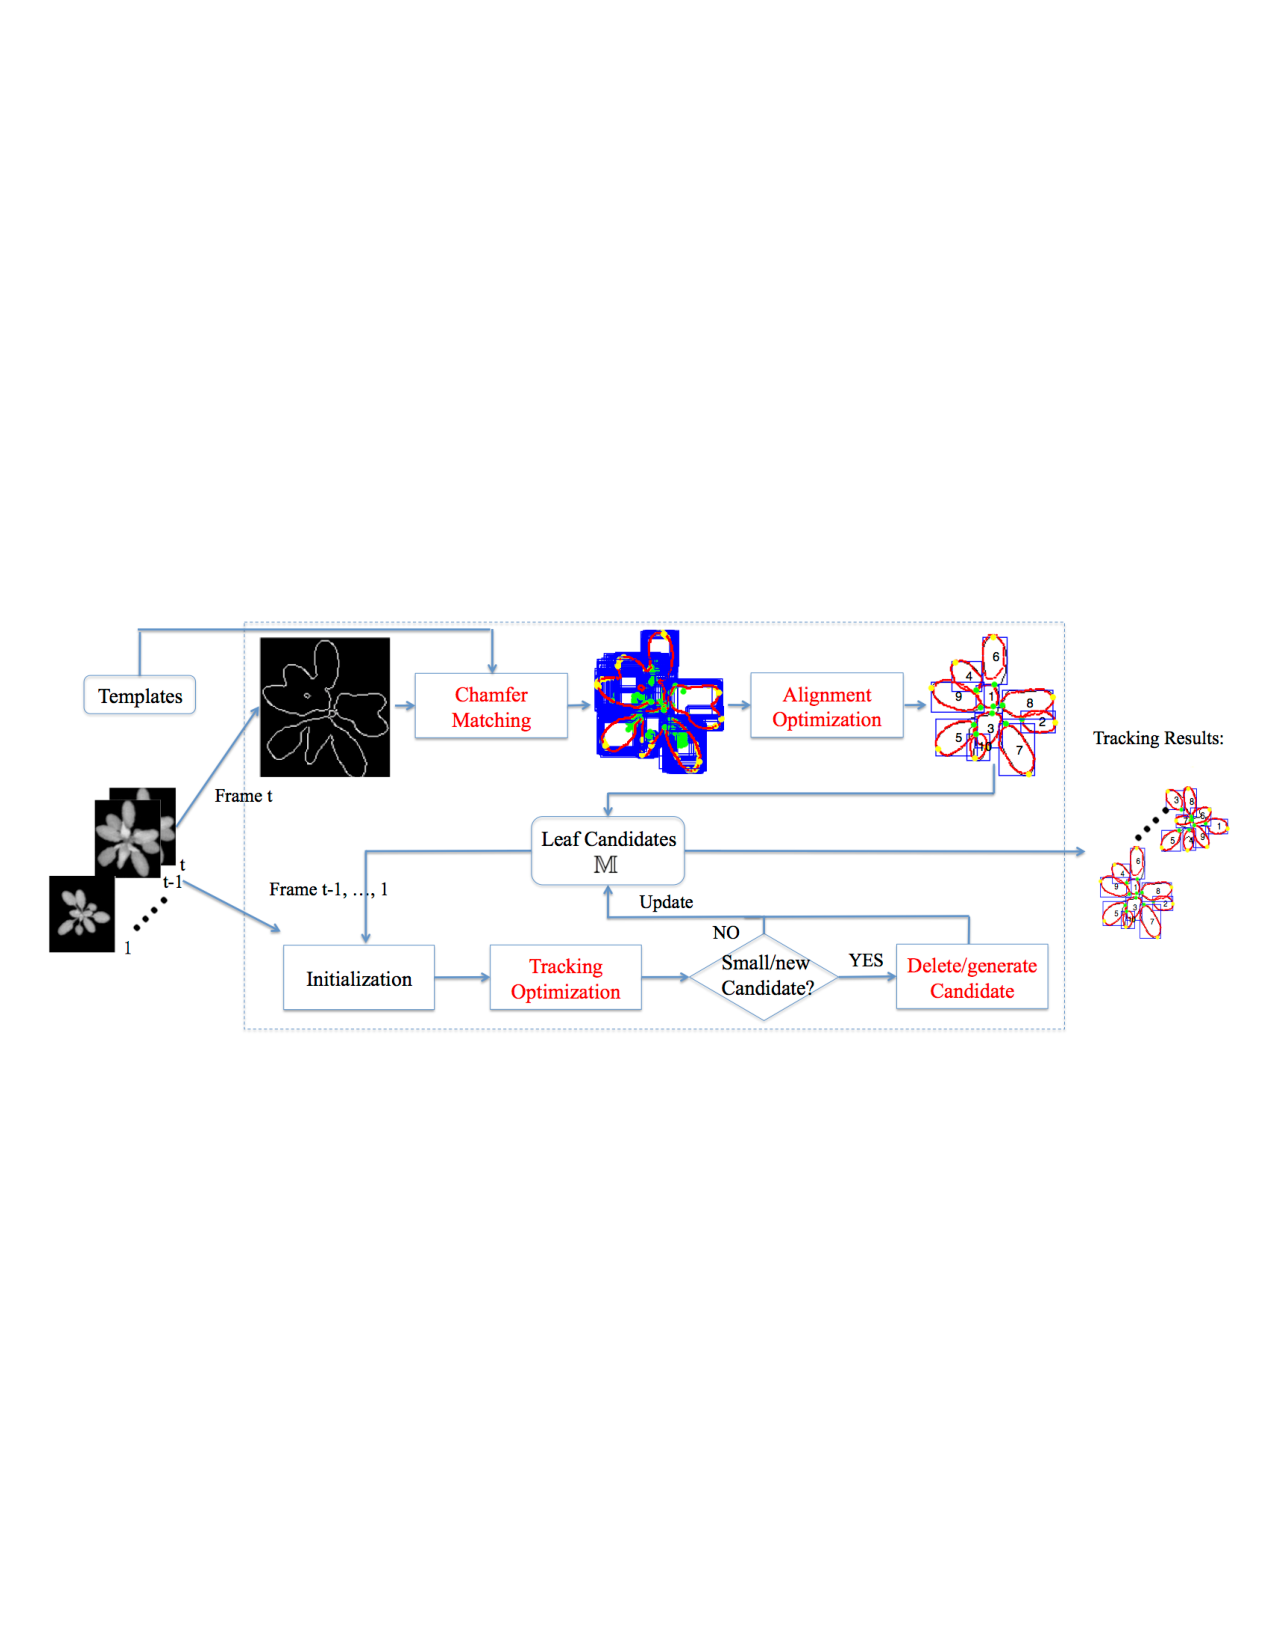
\includegraphics[width=.98\textwidth]{Figures/overview}\\
\caption{Overview of the baseline method.}
\label{fig:methodOverview}
\end{figure*}

\subsection{Experimental Protocols}
\label{sec:protocol}
As shown in Table~\ref{tab:database}, MSU-PID can be used for applications such as leaf segmentation, leaf counting, leaf alignment, and leaf tracking.
To facilitate future research, we separate the database into training set and testing set.
$40\%$ of the data is used for training and $60\%$ for testing.
Specifically, $6$ plants of Arabidopsis and $2$ plants of bean are selected for training.
%We will provide training and testing data in different folders.
For fair comparison, both supervised learning and unsupervised learning methods should evaluate their performance on the training and testing sets separately.

The user may decide to utilize one or multiple modalities of the plant imagery for training and testing respectively.
The availability of multiple modalities allows user to design novel experimental setup.
For example, using RGB and depth modalities for training and RGB for testing can take advantage of additional information during the learning without incurring extra sensor cost during the testing, which can be implemented via either learning with side information~\cite{chen2013boosting}, or transfering learning with missing modality~\cite{ding2014latent}.


\paragraph{Performance Metric}
To evaluate the performance of leaf segmentation, alignment, tracking, and counting, we use four performance metrics, whose Matlab implementations will be provided along with the data.
Three of them are based on the tip-based error, which is defined as the average distance of a pair of estimated leaf tips $\hat{\bm{t}}_{1,2}$ with a pair of labeled leaf tips $ \bm{t}_{1,2}$ normalized by the labeled leaf length:
\begin {equation}
e_{la}(\hat{\bm{t}}_{1,2}, \bm{t}_{1,2}) = \frac{||\hat{\bm{t}}_1-{\bm{t}}_1||_2 + ||\hat{\bm{t}}_2-{\bm{t}}_2||_2}{2 ||\bm{t}_1-\bm{t}_2||_2}.
\label{eqn:tipError}
\end{equation}

We build the frame-to-frame and video-to-video correspondence respectively and generate two sets of tip-based errors.
More details can be find in~\cite{yin2015}.
We define a threshold $\tau$ to operate on the corresponding tip-based errors.
By varying $\tau$, we compute the first three metrics as follows:
\begin{itemize}
\item {\it{Unmatched Leaf Rate (ULR)}}, the percentage of unmatched leaves with respect to the total number of labeled leaves.
This can attribute to two sources.
The first is miss detections and false alarms.
The second is matched leaves with tip-based errors larger than $\tau$.
When $\tau$ is large enough, this value is equal to the leaf counting error.
\item {\it{Landmark Error (LE)}}, the average tip-based errors smaller than $\tau$ of all frame-to-frame correspondent leaves.
This is used to measure the leaf tip alignment error.
\item {\it{Tracking Consistency (TC)}}, the percentage of video-to-video correspondent leaves whose tip-based errors are smaller than $\tau$.
This is used to measure leaf tracking accuracy.
\end{itemize}

In order to evaluate the leaf segmentation accuracy, we adopt an additional metric~\cite{scharr2014annotated} based on the Dice score of estimated segmentation results and ground truth labels:
\begin{itemize}
\item {\it{Symmetric Best Dice (SBD)}}, the average symmetric best Dice among all labeled leaves.
\end{itemize}
The Matlab function for computing {\it{SBD}} is provided by~\cite{scharr2014annotated}.
%The instructions on how to use the evaluation functions are included as comments of the function.


%For leaf annotation, we use the idea of merging and splitting super pixels.
%There are six different numbers of super pixels: $100$, $200$, $300$, $500$, $800$, $1000$.
%The user can specify which level to use depending on how well the super pixels can separate the leaves from the background.
%Because one leaf can be covered by several super pixels and one super pixel can across two leaves or the foreground and background.
%We allow merging and splitting super pixels.
%Merging is implemented by drawing a rectangle on the image.
%Every super pixel overlapping with this rectangle will be merged together.
%Splitting is implemented by drawing a line separating a leaf from the background or from another leaf.
%
%As shown in Figure ~\ref{fig:label}, several super pixels that covers one leaf are first merged together to form a large super pixel.
%Since the top part of the super pixel covers some of the background and the bottom part covers another small leaf, two lines are drawn on this super pixel to split it.
%The leaf boundary is overlaid on the image for better visualization to guide the next action.
%This process continues until all leaves have been annotated.
